\chapter{State of the art}
\label{chap:stateoftheart}

\section{Deployment tool for an UAV network}
\label{chap:stateoftheart:deploymenttool}

The tool is also able to calculate a more precisly pathloss since 


The calculation of electromagnetic radiation require several input values which need to be known. To fullfill this, a deployment tool developped by
The WAVES research group at UGent has therefore developed a deployment tool which distributes UAVs equiped with femtocell base stations. These kind of UAVs will be called 
a \gls{UABS}. 

A deployment tool for an UAV-aided emergency network is described in \cite{J2}. The idea is that in case of a disaster, the existing network might be damaged and won't be able 
to handle all users who are trying to reconnect to the backbone network. A fast deployable network is suggested in \cite{J2} by using \gls{UABS}s. These are UAVs equiped with femtocell base stations
and will be distributed over the disaster area, orchestrated by the deployment tool. 

%The optimal placement for each \gls{UABS} needs to be defined to make sure that as many users as possible are properly reconnected to the backbone network while satisfying certain restrictions. 
%To make these calculations as realistic as possible the architecture of the several buildings present in the area is described in a shapefile. 
%A deployment tool calculates the optimal position of the \gls{UABS} by taking the 3D models of the building into account along with some femtocell specifications and user distribution. This deployment tool is developed by the WAVES research group, a department within Ghent University.

The deployment tool will try to calculate the optimal placement for each \gls{UABS} and requires therefore a description of the area where the UAV-aided network needs to 
be deployed. This is done with the use of so-called shape files. Theses files contains tree dimensional descriptions of the buildings present in the area and are
key values in approaching results as realistic as possible. Furthermore, the tool also requires a time period and a configuration file containing technical specifications of the type of \gls{UABS} that is being used. 
The tool will thereafter randomly distribute users over the area and assigns a certain bitrate to them. \\
\\
In a second phase, the optimal possition for each \gls{UABS} is calculated. This is done by trying to locate a \gls{UABS} above each active user. Two options are possible.
If a flighheigt is defined, a basestations is placed above each user at the given height, unless a building is abstructing it's location. Then, no basestation will be located above that user.
If no flighheigt is given to the tool, the basestation is located 4 meters above the outdoor user or 4 meters above the building where the indoor user resides. 
The later is only allowed if the suggested heigt remains below the given maximum allowed height. \\
\\
Finally, all  \gls{UABS} are sorted on wether they were active or not, followed by the increasing pathloss from each \gls{UABS} to that user.
So the algirtm starts by checking for each active \gls{UABS} if it can cover the user. If this is the case, the user will be connected to this \gls{UABS}. If not,
the second active basestation with a (slightly) worse pathloss is considered. If no active basestation is suitable, inactive \gls{UABS} are considered. The user remains uncovered if no \gls{UABS}
is found. The reasoning behind first only considering basestations that are already active is the hight cost that comes allong with each drone. \\
\\
Up till now, the tool has only calculated some suggestions. The effective provisioning is done in the fourth phase where drones are sorted by the ammount of users it covers. As long as \gls{UABS}
are available in the facility where they reside, \gls{UABS} are provisioned and its users are marked as covered.


\section{Electromagnetic exposure}

\subsection{Electromagnetic field radiation} % (fold)
\label{sub:emf}
People in a telecommunication network are exposed to far field electromagnetic radiation originating from basestations and other \gls{UE}. 
Network planners need to make sure that the the electromangteic fields (expressed in V/m) does not exceed limitations enforced 
by the government. These limits are location dependend. The \gls{ICNIRP} suggests a limitation of 61 V/m. In Brussels, for example, 
is a far more restrictive limitation enforced of 6 V/m for all sources \cite{J1, J10_RDP}.

todo: gedetailleerde uitleg in J23.


\subsection{Specific absorption rate}

\gls{SAR} represents the rate that electromagnteic energy is absorption by human tissue with the thermal effect as it's most important consequence.
The \gls{ICNIRP} has concluded that the threshold effect is at 4 W/kg meaning that any higher absorption rate would overwhelm thermoregulatory capacity of the human body.
Whole body values between 1 and 4 W/kg increases the temparture of human body less then 1°C which is proven not to be harmfull for a healthy human being\cite{J24}.
Thereafter, a safety margin is introduced to tackle unknown variables like experimental errors, increased sensitivity for certain population groups and so on. This results 
in a whole body $SAR_{10g}$ of $0.8 W/kg$ and $2 W/kg$ for localized $SAR_{10g}$ values for the head and torso aera \cite{J23}.

todo: de 10g slaat al op localized, vandaar dat het maar 10g is, anders is het whole-body
todo: we kunnen niet sar10gmax gebruiken want This means that the SAR calculations will be worst-case and possibly an overestimation of the real localised SAR. (herwoorden voor plagiaat)
Human exposure caused by downlink traffic is a not negligible asset. However, telecommunications is not a one-way street. When connecting to a UMTS network, also uplink data caused by the \gls{UE} should be considered.
\gls{UE} generates, just like femtocells, electromagnetic waves to which a user is exposed. A part of this radiation goes to the femtocell, another part enters the body of its user. How much electormagnic strenghts enters the body is defined as \gls{SAR} and is measured with 10g biological tissue which represents the human skin. This value will from now on be expressed as $SAR_{10g}$. 
A mobile device induces two types of exposure: local and whole-body. 



\subsection{Related work} % (fold)
\label{sub:general}
The goals of this master dissertation is the investigation of electromagnetic exposure considering all sources. Three types of sources are considered: electromagnetic radiation 
caused by basestations, near field radiation from the users own device and far field radiation originating from other users their equipment. This electromagnetic radiation is thereafter
absorbed by the human body which will be expressed in \gls{SAR} values. Different type of \gls{SAR}-values exist like whole body \gls{SAR} which is the average absobed radiation over the entire 
body. Also more precise \gls{SAR}-values exist which go under the name of localized \gls{SAR}-values and only cover a part of the human body like the head.

Several papers exist calculating exposure originating from certain sources but very limited research has been done covering the whole picture.
In \cite{J6_originalExposureFormula} is described how electromagnetic radiation of several WiFi access points is being calculated. The authors of \cite{J1} used this knowledge 
to investigate electrmangetic exposure originating from basestations in a more outdoor environment. \cite{J10_RDP, J10.1} addresses the fact that 
also \gls{UL} traffic from the user's device should be considered. They therefore investigated indoor exposure. They did not only consider the electromagnetic radiation
but also how much is absorbed by the body wich will be expressed as specific absorption rate. Since the authors only covered voice calls,
uplink SAR was expressed in localized SAR values while the downlink traffic is expressed in whole body SAR. With the advent of 5G, a paper \cite{J17_kuehn2019modelling} has been 
published describing how localized SAR values are achieved from all sources. More precisly: all mobile phones and all basestations in the network after which they converted the electromagnetic 
exposure to localized SAR values.
Finally, \cite{J22_plets2015joint} describes how both \gls{UL} and \gls{DL} traffic can be converted in whole body SAR values making it possible to achieve an overall picture. They applied this formula 
howevery only for the user's own device.

In a realistic network like the used deployment tool, some users are calling while annother part is using other type of telecommunication services like browsing the web.
Therefore, all absorbed electromagnetic exposure should be expressend in whole body SAR while still covering all sources.


\section{Optimizing towards electromagnetic exposure and power consumption}
todo: leg uit Dat de twee omgekeerd evenredig zijn.



\section{Technologies}
\subsection{LTE}
The tool make usage of \gls{LTE} which is by the general public better known as 4G which allowes better \gls{UL} and \gls{DL} dataspeeds 
compared to its predecessors and is based on an all IP architecture. LTE can cover macrocells supporting cell sizes ranging from 5 km up to 100 km. 
These type of antennas are usally attached to transmission towers along highways or on top of buildings. LTE supports however also smaller cells like
femtocells covering only a few hunderd meters. They are therefore more portable, require less energy and won't require a telecommunication operator because
of it's simplicity. Femtocell basestations are therefore used by the deployment tool.
Futher, \gls{LTE} also support both \gls{FDD} and \gls{TDD}.

\gls{FDD} makes simultanious \gls{UL} and \gls{DL} traffic possible by assiging different frequencies within the frequency range 
to both data streams. A small guardband is used between \gls{UL} and \gls{DL} directions in other to prevent interference.

\gls{TDD} allowes  \gls{UL} and \gls{DL} by splitting the time domain. Meaning that both traffic directions use the same frequency and therefore
alternatly (in time) use the frequency spectrum. Again, a small time intervall is used to prevent interference in case of a slightly bad timed syncronization.

This master dissertation will make usage of \gls{FDD}.


\subsection{Type of antenna} % (fold)

An important part of this master dissertation is the type of antennas that will be used by the basestations. Since the deployment tool make usage
of drones in other to possition the femtocell basestations in the right posistion,  conventional 
sector antennas as used by terestrial transmission towers won't be a good idea. The characteristics of microstrip antennas will therefore be investigaged.

Microtstrip anntenas provide several advantages compared to traditional antennas \cite{J13_singh2011micro, J14_antennadesign}. Microstrip antennas
are lightweight, low in cost and thin causing them to be more aerodynamic which is  a usefull feature since the atennas will be attached
to flying drones.

A basic microstrip antenna like figure \ref{fig:basicpatchantenna} consisting a ground plane and
a radiating patch which are seperated with a dielectric substrate. Several constructions exist like microstrip patch antenna, microstrip slot antenna and printed dipole antenna which
has all similar characteristics. They are all thin, support dual frequency operation and they all have the dissadvatage of \gls{spuriousradiation}.The microstrip patch and slot antenna support both linear
and circular polarization while the printed dipole only support linear polarization. Further is the fabrication of a microstrip patch antenna considered to be the easiest of its competitors. 



\begin{figure}[H]
  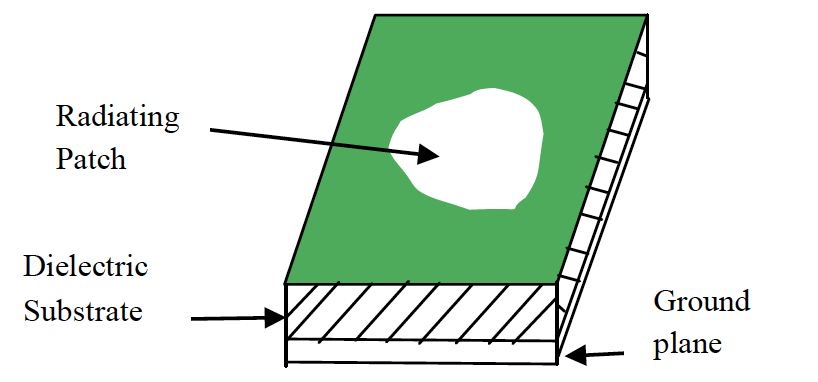
\includegraphics[width=\textwidth/2]{../images/patchantenna.png}
  \caption{General design of a microstrip antenna}
  \label{fig:basicpatchantenna}
\end{figure}


The microstrip antenna requires besides the groundplane, dielectric substrate and the radiation pach also a feed line. Several feeding techiques exists of which the most popular are: coaxial probe feeding, microstrip line and apeture coupling. %and Microstrip Patch Antenna
(todo: more refs? gebruik nummer twee van J13 (p2))

A first feeding method is with the usage of a coaxial cable where the outer conductor is attached to the ground plane and the inner conductor to the radiationg patch. Modelling is however difficult, escpecially for thic substrates as will be used in this master dissertation.
A second option is the usage of a microstrip line. This type of feeding is much easier to model since the microstrip line can be seen as en extenstion of the radiating patch. A dissadvatage is that the antenna will transmit at frequencies outside the aimed band which
is also known as \gls{spuriousradiation} which therefore  limits bandwith.
A thirt is proximity coupling which has the largest bandwidth and low \gls{spuriousradiation}. It consist however of two dielectric substrates causing the overall thickness
of the antenna to increase as well as it's fabrication difficulty.
(todo: tekst te weinig, bespreek ook apperture coupled attenna (zelfde paper als de rest))
The increasing usage of the microstrip patch antennas can be explained by it's easy fabrication and lightweightness and therefore knows a widespread application in the millitary, global possitioning systems, telemedicine and WiMax applications and so on.
The authors also state that some of the dissadvatages like lower gain and power handling can be solved with the usage of an array configuration.

At last, also the materials of the antenna need to be considered. The radiationg patch mainly rectengular. In fact is any given shape possible but other configurations
then a cirle or a rectangle will require large nummerical computation \cite{J14_antennadesign}. The radiating patch is usualy made of a thin layer of either gold or copper \cite{J14_antennadesign,J15_antennadesign}. 
Further is also the dielectric constant of the substrate important which typially varies between 2.2 and 12. Finding a good dielectric depends how the antenna will be deployed and it's usage. According to  \cite{J15_antennadesign} will a lower
dielectric constant with a thic substrate result in better performance, better efficiency and larger bandwiths. On the other hand will according to \cite{J14_antennadesign} a larger dielectric constant reduce de dimensions of the antenna which is also usefull when attaching the 
antenna to a limited surface. Therefore is opted for a glass as dielectric substrate with a constant of 4.4.

